\documentclass[addpoints,12pt]{exam}
\usepackage{amsmath, amssymb}
\linespread{1.1}
\usepackage{graphicx}
\usepackage{multirow}
\usepackage{moreverb}
\boxedpoints
\pointsinmargin
\usepackage[T5,T1]{fontenc}  


%\printanswers
%\noprintanswers

\pagestyle{headandfoot}
\runningheadrule
\runningheader{Econ 103}
              {Final Examination, Page \thepage\ of \numpages}
              {May 4th, 2017}

\runningfooter{Name: \rule{5cm}{0.4pt}}{}{Student ID \#: \rule{5cm}{0.4pt}}


%%%%%%%%%%%%%%%%%%%%%%%%%%%%%%%%%%%%%%%%%%%%%%%%%%%%%%%%%%%%%%%
\begin{document}

\begin{center}
\large
\sc{Final Examination\\ \normalsize Econ 103, Statistics for Economists \\ \vspace{0.5em} May 4th, 2017}

\vspace{1em}

\normalsize
\fbox{\begin{minipage}{0.51\textwidth}
\textbf{\small You have 120 minutes to complete this exam.
Graphing calculators, notes, and textbooks are not permitted. }\end{minipage}}


\end{center}
%%%%%%%%%%%%%%%%%%%%%%%%%%%%%%%%%%%%%%%%%%%%%%%%%%%%%%%%%%%%%%%


\vspace{2em}
\begin{center}
  \fbox{\fbox{\parbox{5.5in}{\centering
        I pledge that, in taking and preparing for this exam, I have abided by the University of Pennsylvania's Code of Academic Integrity. I am aware that any violations of the code will result in a failing grade for this course.}}}
\end{center}
\vspace{0.2in}
\makebox[\textwidth]{Name:\enspace\hrulefill}

\vspace{0.2in}
\noindent \makebox[\textwidth]{Student ID \#:\enspace\hrulefill}

\vspace{0.3in}
\noindent\makebox[\textwidth]{Signature:\enspace\hrulefill}

%\rule{1cm}{0.4pt}
\vspace{2em}

\begin{center}
  \gradetable[h][questions]
\end{center}

\vspace{2em}

\paragraph{Instructions:} Answer all questions in the space provided, continuing on the back of the page if you run out of space. Show your work for full credit but be aware that writing down irrelevant information will not gain you points. Be sure to sign the academic integrity statement above and to write your name and student ID number on \emph{each page} in the space provided. Make sure that you have all pages of the exam before starting.

\paragraph{Warning:} If you continue writing after we call time, even if this is only to fill in your name, twenty-five points will be deducted from your final score. In addition, two points will be deducted for each page on which you do not write your name and student ID. 

%%%%%%%%%%%%%%%%%%%%%%%%%%%%%%%%%%%%%%%%%%%%%%%%%%%%%%%%%%%%%%%
\newpage

\begin{questions}


  \question[35] Mars inc.\ produces the ``colorful button-shaped chocolates'' M\&M's.
  The contents of a bag of M\&M's changed in 1995 when tan M\&M's were replaced by blue M\&M's.
  The relative frequencies of the remaining colors changed as well.
  The values you will need to solve this problem appear in bold in the following table:
  \begin{center}
    \begin{tabular}{c|ccccccc}
      & blue & tan & \textbf{green} & orange & \textbf{yellow} & \textbf{red} & brown \\
      \hline
      Before 1995 (\emph{Old}) & -- & 10\% & \textbf{10\%} & 10\% & \textbf{20\%} & \textbf{20\%} & 30\% \\
      After 1995 (\emph{New}) & 24\%& -- & \textbf{20}\% & 16\% & \textbf{14\%} & \textbf{13\%} & 13\%
    \end{tabular}
  \end{center}
  I have two bags of M\&M's: one from before 1995 (\emph{Old}) and one from after 1995 (\emph{New}).
I randomly choose a bag, such that each is equally likely to be selected.
I then make three independent random draws with replacement from the bag. 
I obtain: green, yellow, red.
Given this information, what is the probability that I selected the \emph{Old} bag?
%Let $Old$ be the event that I drew the old bag and $New$ be the event that I drew the new bag. 
%Similarly, let $G$ denote the event that I drew a green, $Y$ a yellow, and $R$ a red M\&M. 
\begin{solution}[6in]
First, by the law of total probability, we have
\[P(G,Y,R) = P(G,Y,R|O)P(Old) + P(G,Y,R|N)P(New)\]
Since I make my draws independently with replacement,
\begin{align*}
P(G,Y,R|Old) &= P(G|Old)P(Y|Old)P(R|Old)\\
&= 1/10 \times 1/5 \times 1/5 = 1/250
\end{align*}
and similarly
\begin{align*}
P(G,Y,R|New) &= P(G|New)P(Y|New)P(R|New)\\
&= 1/5 \times 14/100 \times 13/100 = 182/50000
\end{align*}
Thus,
\[P(G,Y,R) = 1/250 \times 1/2 + 182/50000 \times 1/2\]
and by Bayes' Rule,
\begin{align*}
  P(Old|G,Y,R) &= \frac{P(G,Y,R|Old)P(Old)}{P(G,Y,R)}\\
  &= \frac{1/250 \times 1/2}{1/250 \times 1/2 + 182/50000 \times 1/2}\\
  &= \frac{1/250}{1/250 + 182/50000} = \frac{200}{200 + 182}= 100/191 \approx 0.52
\end{align*}
\end{solution}

  \question The $\chi^2(m)$ is a random variable that we did not study in lecture this semester. 
  If $Z_1, \dots, Z_m \sim \mbox{iid } N(0,1)$ then $Y = Z_1^2 + Z_2^2 + \cdots + Z_m^2$ is a $\chi^2(m)$ RV.
  In other words the $\chi^2(m)$ RV is the \emph{sum of squares} of $m$ iid standard normal RVs.
  The $\chi^2(m)$ RV has a single parameter: the \emph{degrees of freedom} $m$.
  R has a built-in function \texttt{rchisq} for making random draws from a $\chi^2(m)$ distribution.
  In this question we will create our own version: \texttt{myrchisq}.
    In your answers you may use any R functions \emph{except} \texttt{rchisq}.
  \begin{parts}
    \part[10] Create an R function called \texttt{draw\_chisq} that constructs a single draw from a $\chi^2(m)$ random variable by making $m$ iid standard normal draws and calculating their sum of squares.
    Your function should take a single input argument -- the degrees of freedom $m$ -- and return the $\chi^2(m)$ random draw.
    \begin{solution}[1.5in]
      \begin{verbatim}
draw_chisq <- function(m){
  x <- rnorm(m)
  return(sum(x^2))
} \end{verbatim}
    \end{solution}
    \part[10] Create an R function called \texttt{myrchisq} that repeatedly calls \texttt{draw\_chisq(m)} to generate $n$ iid draws from a $\chi^2(m)$ distribution.
    It should take two inputs -- the number \texttt{n} of $\chi^2$ draws, and degrees of freedom \texttt{m} -- and return a vector of $n$ iid $\chi^2(m)$ draws.
    \begin{solution}[1.2in]
      \begin{verbatim}
myrchisq <- function(n, m){
  out <- replicate(n, draw_chisq(m))
  return(out)
} \end{verbatim}
    \end{solution}
    \part[10] Write R code that uses \texttt{myrchisq(n,m)} to approximate the probability that a $\chi^2(1)$ RV takes on a value strictly greater than 4 using 10,000 Monte Carlo simulations.
    \begin{solution}[1in]
      \begin{verbatim}
sims <- mychisq(10000, 1)
mean(sims > 4) \end{verbatim}
    \end{solution}
    \part[5] Using what you know about the standard normal RV, approximately what would be the numeric result of running your code from part (c)?
    \begin{solution}[1in]
      A $\chi^2(1)$ RV is just the square of a standard normal RV $Z$.
      Thus $P(\chi^2(1) > 4) = P(Z^2 >4) = P(Z<-2 \mbox{ or } Z>2) \approx 0.05$.
    \end{solution}
  \end{parts}

  \question Let $Y_1, Y_2, Y_3 \sim \mbox{ iid } N(0, \sigma^2 = 36)$ and define: $\displaystyle Z = Y_1 + \frac{Y_2}{2} + \frac{Y_3}{3}$.
  \begin{parts}
    \part[5] Calculate $E[Z]$
    \begin{solution}[1.5in]
      By the linearity of expectation
      \[E[Z] = E[Y_1] + \frac{E[Y_2]}{2} + \frac{E[Y_3]}{3}=0\]
    \end{solution}
    \part[5] Calculate $\mbox{Var}(Z)$
    \begin{solution}[1.5in]
      Since $Y_1, Y_2$, and $Y_3$ are iid
      \[\mbox{Var}(Z) = \mbox{Var}(Y_1) + \frac{\mbox{Var}(Y_2)}{4} + \frac{\mbox{Var}(Y_3)}{9} = \frac{49}{36}\times 36= 49\]
    \end{solution}
    \part[5] What kind of random variable is $Z$? Specify the values of any and all parameters.
    \begin{solution}[1.5in]
      Linear combinations of independent normals random variables are normal, hence $Z\sim N(0, 49)$.
    \end{solution}
    \part[10] For what value of $c$ is $P(Z<c)\approx 0.975$? Your answer should specify a numeric value and not rely on any R commands.
    \begin{solution}[2in]
      Since $P(Z<c) = P(Z/7 < c/7)= \texttt{pnorm}(c/7)$, we need to solve for $c$ such that $\texttt{pnorm}(c/7) \approx 0.975$.
      Taking \texttt{qnorm} of both sides, we have $c/7 \approx \texttt{qnorm}(0.975)$ so $c \approx 14$.
    \end{solution}
  \end{parts}


  \newpage
  \uplevel{\emph{The following question is taken verbatim from your Homework for Lectures 16--17.}}

\question This question is based on a recent paper examining how ``organic'' labeling changes people's perceptions of different food products. Researchers recruited volunteers at a local mall in Ithaca, New York and gave each two samples of yogurt to taste. Although both yogurts were in fact identical, the volunteers were \emph{told} that one of them was organic while the other was not. After tasting both, each volunteer was asked to estimate how many calories each of the samples of yogurt contained. (Since, unknown to the volunteer, both samples contained exactly the same kind of yogurt, each in fact contained the same number of calories.) To prevent confounding from anchoring or other behavioral effects, the order in which a given volunteer tasted the two yogurts, i.e.\ ``organic'' first or ``organic'' second, was chosen at random. The results of this experiment are stored in an R data table called \texttt{yogurt}. Here are the first few rows:
	\begin{verbatim}
> head(yogurt)
	  regular organic
1      60      40
2       5       0
3     200     100
4      60      40
5     100     100
6      90      90
	\end{verbatim}
Each row in this data table corresponds to a single individual's guess of the number of calories contained in each of the two yogurts. For example, the values 60 and 40 in row 1 mean that volunteer number one guessed that the regular yogurt sample contained 60 calories and the organic sample contained 40. Summary statistics for the two columns are as follows:
	\begin{center}
		\begin{tabular}{|lcc|}
		\hline
			& \texttt{regular} & \texttt{organic}\\
			\hline
		Sample Mean & 113 & 90\\
		Sample Var & 3600 & 2916\\
		Sample SD & 60 & 54\\ 
		Sample Corr.\ &\multicolumn{2}{c|}{0.8} \\
		Sample Size &\multicolumn{2}{c|}{115} \\
		\hline
		\end{tabular}
	\end{center}
	\vspace{1em}
	\begin{parts}
		\part[8] Give the units of each of the summary statistics from above:\\
		
			\begin{tabular}{lc}
			Sample Mean &\underline{\makebox[1.5in][l]{}} \\
			Sample Var.\ &\underline{\makebox[1.5in][l]{}}\\
			Sample SD& \underline{\makebox[1.5in][l]{}}\\
			Sample Corr. & \underline{\makebox[1.5in][l]{}}\\
			\end{tabular}
			\begin{solution}
			calories, calories$^2$, calories, unitless.
			\end{solution}
		\part[6] Sara thinks that this experiment should be analyzed as independent samples data. Assume that she is correct and construct an approximate 95\% CI for the difference of means (\texttt{regular} - \texttt{organic}) based on the CLT.
			\begin{solution}[2in]
			The difference of means (regular minus organic) is 23 calories. Sara calculates her standard error assuming independent samples:
			$$\sqrt{\sigma^2_X/n + \sigma^2_Y/m} = \sqrt{3600/115 + 2916/115} = \sqrt{6516/115} \approx 7.5$$
			so her confidence interval is approximately $23 \pm 15$, in other words $(8,38)$.
			\end{solution}
		\part[6] Kevin thinks that this experiment should be analyzed as matched pairs data. Assume that he is correct and construct an approximate 95\% CI for the difference of means (\texttt{regular} - \texttt{organic}) based on the CLT.
		\begin{solution}[2in]
		Kevin takes into account the sample correlation between columns when calculating his standard error. He does this by using the sample statistics from the table to calculate the sample variance of the \emph{differences}: regular minus organic. In particular, he calculates:
		$$s^2_D =  3600 + 2916 - 2 \cdot 0.8 \cdot 60 \cdot 54 = 1332$$
		which gives a standard error of
		$$\sqrt{s_D^2/n} = \sqrt{1332/115} \approx 3.4$$
		This is the only difference between his procedure and Sara's. Hence, Kevin's confidence interval is approximately $23 \pm 6.8$, in other words $(16.2, 29.8)$.
		\end{solution}
		\part[6] How do the confidence intervals constructed by Sara and Kevin differ? What is the reason for this difference? Who has has constructed the appropriate confidence interval for this example: Kevin or Sara? Explain briefly. 
		\begin{solution}[2.5in]
		Kevin is right and Sara is wrong. This is matched pairs data because each row corresponds to a \emph{single individual}. Unsurprisingly, we find a high sample correlation between the two columns: individuals who overestimate caloric content for one yogurt sample tend to do so for the other, as do individuals who underestimate. The only difference between Kevin and Sara's confidence intervals comes from how they calculated their standard errors. Both intervals are correctly centered, but Sara's is \emph{too wide} because she calculated the standard error assuming independence between the two samples. When the sample correlation is positive this results in an \emph{overestimate} of the standard error. 
		\end{solution}
		\part[6] Suppose that Kevin wanted to carry out a two-sided test of the null hypothesis that organic labeling does not affect consumer's estimates of caloric content, on average. What is his test statistic? What R command should he use to calculate the p-value for his test? Will his result be greater or less than 0.05? 
		\begin{solution}[2.75in]
		Kevin's test statistic is the difference of means divided by the standard error, namely $23/3.4 \approx 6.8$. To calculate the p-value in R, he should use the command:
			$$\texttt{2 * (1 - pnorm(6.8))}$$
			The result will be less than 0.05 since the test statistic is larger than 2. Another way to see this is that his confidence interval does not include zero.
		\end{solution}
		\part[8] Using your knowledge of experiments, observational studies, hypothesis testing, and confidence intervals, what conclusions can we draw from this study? Explain briefly.
		\begin{solution}[4.5in]
		It appears that merely labeling a product ``organic'' causes consumers to assume that this product contains fewer calories. Because this is a randomized experiment (randomly assigning labels to identical samples of yogurt and randomizing the order in which subjects tasted), we don't have to worry about confounding. It is less clear, however, whether this result would generalize to foods other than yogurt. Further, people from Ithaca New York who visit the mall and volunteer for a taste test may not be representative of US consumers as a whole. Ideally we would repeat this experiment using different subject pools and different foods to see how robust the result is.
		\end{solution}
	\end{parts}

  \question Let $X_1, \dots, X_n\sim \mbox{ iid Bernoulli}(p)$ and define $\widehat{p} = \sum_{i=1}X_i/n$.
  This question concerns a test of $H_0\colon p = 0.5$ against $H_1\colon p>0.5$ with $\alpha = 0.025$.
  \begin{parts}
    \part[5] If $p = 0.5$ and $n$ is large, what is the approximate sampling distribution of $\widehat{p}$?
    \begin{solution}[1.7in]
      By the Central Limit Theorem, if $n$ is large then $\widehat{p}$ is approximately normal with mean $p=0.5$ and variance $\displaystyle \frac{p(1-p)}{n} = \frac{1}{4n}$.
    \end{solution}
    \part[5] Write down the test statistic $T_n$ for the test specified in the problem statement. 
    Be sure to fully impose the null hypothesis.
    \begin{solution}[1.7in]
      $\displaystyle T_n = \frac{\widehat{p} - 0.5}{\sqrt{1/4n}} = \sqrt{n}(2\widehat{p} - 1)$
    \end{solution}
    \part[5] If $p=0.5$ and $n$ is large, approximately what is the sampling distribution of the test statistic from part (b)?
    Using this information, what is the critical value and decision rule for the test in the problem statement?
    \begin{solution}[1.6in]
      If $p = 0.5$ and $n$ is large then $T_n \approx N(0,1)$. The critical value is approximately $2$ and our decision rule is to reject $H_0$ when $T_n > 2$.
    \end{solution}
    \part[5] If $p=0.5$ what is the probability that we will reject $H_0$? Explain briefly.
    \begin{solution}[1.6in]
      Since $p=0.5$ under the null, this probability is simply the type I error rate, which is equal to $\alpha$. For this test the question specifies $\alpha=0.025$.
    \end{solution}
    \part[5] If $p = 0.8$ and $n$ is large, what is the approximate sampling distribution of $\widehat{p}$?
    \begin{solution}[2in]
      By the Central Limit Theorem, if $n$ is large then $\widehat{p}$ is approximately normal with mean $p=0.8$ and variance $\displaystyle \frac{p(1-p)}{n} = \frac{4}{5} \times \frac{1}{5} \times \frac{1}{n} = \frac{4}{25 n}$.
    \end{solution}
    \part[10] Based on your answer to part (e), if $p=0.8$ and $n$ is large, what is the approximate sampling distribution of the test statistic $T_n$ constructed in part (b)? 
    \begin{solution}[2.5in]
      From (a), $T_n = \sqrt{n}(2\widehat{p} - 1) = 2\sqrt{n}\widehat{p} - \sqrt{n}$ which is simply a linear combination of $\widehat{p}$.
      From (e) we know that when $n$ is large and $p=0.8$ the sampling distribution of $\widehat{p}$ is approximately normal with mean $4/5$ and variance $4/(25n)$.
      It follows that the sampling distribution of $T_n$ is approximately normal with mean $2\sqrt{n} \times 4/5 - \sqrt{n} = 3\sqrt{n}/5$ and variance $(2\sqrt{n})^2 \times 4/(25n) = 16/25$.
    \end{solution}
    \part[10] Continuing from part (f), if $p=0.8$ for what value of $n$ is the power of the test in the problem statement approximately equal to 0.84? 
    \begin{solution}[3in]
      The power of the test is the probability of rejecting $H_0$ and our decision rule from part (c) above is to reject when $T_n>2$.
      From part (f), if $p=0.8$ then $T_n \approx N(3\sqrt{n}/5, 16/25)$.
      Hence, we need to solve for $n$ such that
      \begin{align*}
        P(T_n >2) &= P\left( \frac{T_n - 3\sqrt{n}/5}{4/5} > \frac{2 - 3\sqrt{n}/5}{4/5} \right)\\
        &=P\left( Z > \frac{10 - 3\sqrt{n}}{4}\right) \approx 0.84
      \end{align*}
      where $Z \sim N(0,1)$.
      Since we know that $P(Z>-1)\approx 0.84$ for a standard normal we need to solve $(10-3\sqrt{n})/4 = -1$ for $n$.
      Rearranging and solving, we find that $n = 196/9  \approx 22$.
    \end{solution}
  \end{parts}

  \question The data table \texttt{companyX} contains a random sample of 215 employees from Company X: 
\begin{verbatim}
   Male Months Salary
1:    1     91  69250
2:    1     22  53120
3:    0     40  57280
4:    1     88  69830
5:    1     21  56470
6:    0     46  54890
\end{verbatim}
Each row is an employee: \texttt{Male} takes on the value 1 if a given employee is male and zero otherwise, \texttt{Months} gives total months of work experience, and \texttt{Salary} gives annual salary in dollars.
    To answer this question you will need to consult the regression results and plots on the final two pages of this exam. 
    You may want to tear these pages out for convenience.
    For full credit, be sure to clearly reference the specific set of regression results you rely on in each of your answers below. These are numbered 1--4.
  \begin{parts}
    \part[4] Write R code to add a new column to \texttt{companyX} called \texttt{Years} that gives work experience in \emph{years} rather than months: e.g.\ 22 months becomes 1.83 years.
    \begin{solution}[1in]
      \begin{verbatim}
companyX[, Years := Months / 12]
      \end{verbatim}
    \end{solution}
    \part[4] Write the R code needed to generate the boxplots of \texttt{Salary} and \texttt{Years} found on the final page of this exam. You do not have to label the plots.
    \begin{solution}[1in]
      \begin{verbatim}
boxplot(Salary ~ Male, companyX)
boxplot(Years ~ Male, companyX)
      \end{verbatim}
    \end{solution}
    \part[3] 
    Based on the regression results how many years of work experience do the female employees at Company X have on average?
    \begin{solution}[0.85in]
      The intercept from Regression \#2 gives the average number of years of experience of the female employees: 5.44 years.
    \end{solution}
    \part[3] Based on the regression results how much do the male employees at Company X earn per year on average?
    \begin{solution}[0.85in]
      To calculate this, we sum the intercept and the coefficient \texttt{Male} from Regression \#1: $62060 - 3160 = 58900$ dollars.
    \end{solution}
    \part[4] Suppose you had to choose between using \texttt{Male} or \texttt{Years} to predict the salary of an employee at Company X.
    Which appears to give more accurate predictions for the employees in our sample?
    How much more accurate?
    Explain briefly.
    \begin{solution}[1in]
      \texttt{Years} is dramatically more predictive than \texttt{Male}: Regression \#3 predicts to an accuracy of approximately \$3,100 while Regression \#1 predicts to an accuracy of about \$10,300.
    \end{solution}
    \part[6] Suppose we want to test the null hypothesis that male and female employees earn the same salary, on average, against the two-sided alternative with $\alpha = 0.05$.
    Do we reject or fail to reject?
    Explain briefly and show all of your work for full credit.
    \begin{solution}[1.75in]
     To carry out this test, we use the results of Regression \#1.
     The decision rule for this test is to reject if $T_n > 2$.
     The slope of this regression -- \texttt{Male} -- gives the difference of mean salaries: mean minus women.
     Males earn, on average, about \$3,200 less per year with a standard error of about \$1,400.
     Our test statistic is $3200/1400 \approx 2.3$. 
    Since this is larger than $2$, we would reject the null hypothesis.
    \end{solution}
    \part[4] Write R code to make a scatterplot with \texttt{Salary} on the y-axis and \texttt{Years} on the x-axis and plot the corresponding regression line on top of the points.
    \begin{solution}[1in]
      \begin{verbatim}
plot(Salary ~ Years, companyX)
abline(lm(Salary ~ Years, companyX))
      \end{verbatim}
    \end{solution}
    \part[3] Approximately what is the correlation between \texttt{Salary} and \texttt{Experience}?
    \begin{solution}[0.75in]
      This correlation equals the square root of the R-squared from Regression \#3: $\sqrt{0.91} \approx 0.95$
    \end{solution}
    \part[3] What are the units of the slope estimate in Regression \#3? 
    \begin{solution}[0.75in]
      The slope is measured in dollars of annual salary per year of experience.
    \end{solution}
    \part[3] What are the units of the \emph{standard error} of the slope estimate in Regression \#3?
    \begin{solution}[0.75in]
      Since we construct an approximate 95\% confidence interval from Estimate $\pm 2 \times$ SE, the standard error must have the same units as the estimate, in this case dollars of annual salary per year of experience.
    \end{solution}
    \part[3] Is the intercept in Regression \#3 a meaningful quantity? 
    If not, why not? 
    If so, what does it mean?
    Explain briefly.
    \begin{solution}[1in]
      The intercept is meaningful: it gives the predicted annual salary in dollars for an employee with zero years of work experience, i.e.\ someone fresh out of school.
    \end{solution}
    \part[20] Use the statistical tools you have learned in Econ 103 to explain the evidence of a pay gap between male and female employees using the results of Regression \#4.
    Write your answer in bullet points with \emph{no more than five} bullets.
    Clear and succinct responses will be graded more favorably than long, rambling ones.
    \begin{solution}
      Various possibilities, but these are the key points:
      \begin{itemize}
        \item Regression \#4 allows a different intercept and slope for the relationship between \texttt{Years} and \texttt{Salary} between male and female employees.
        \item For females the regression line is $\texttt{Salary} = 41400 + 3800 \times \texttt{Years}$ while for males it is $\texttt{Salary} = 45800 + 3070 \times \texttt{Years}$.
        \item The estimate and standard error for \texttt{Male} indicate that, when comparing a male and female who both have zero previous job experience, we predict that the male earns about \$4400 more per year with an approximate 95\% confidence interval of $4400 \pm 1600$ or $(2800,6000)$ for the difference of intercepts.
        \item The estimate and standard error for \texttt{Male:Years} indicate that male employees are paid about \$730 \emph{less} per year of additional job experience than women with an approximate 95\% confidence interval of $-730 \pm 280$ or $(450,1010)$ for the difference of slopes.
        \item We have found strong statistical evidence of salary differences between male and female employees. 
          Moreover these differences are large in magnitude.
          The overall pattern, however, is complicated: among employees with few years of experience, males are better-paid, but among employees with many years of experience, females are better-paid.
      \end{itemize}
    \end{solution}
  \end{parts}

\newpage
\footnotesize
\paragraph{\footnotesize Regression \#1}
\begin{boxedverbatim}
lm(formula = Salary ~ Male, data = companyX)
            coef.est coef.se 
(Intercept) 62059.27   981.92
Male        -3159.65  1405.07
---
n = 215, k = 2
residual sd = 10298.43, R-Squared = 0.02
\end{boxedverbatim}
\vspace{-1em}

\paragraph{\footnotesize Regression \#2}
\begin{boxedverbatim}
lm(formula = Years ~ Male, data = companyX)
            coef.est coef.se
(Intercept)  5.44     0.27  
Male        -1.17     0.39  
---
n = 215, k = 2
residual sd = 2.86, R-Squared = 0.04
\end{boxedverbatim}
\vspace{-1em}

\paragraph{\footnotesize Regression \#3}
\begin{boxedverbatim}
lm(formula = Salary ~ Years, data = companyX)
            coef.est coef.se 
(Intercept) 43940.75   418.48
Years        3406.18    73.85
---
n = 215, k = 2
residual sd = 3143.62, R-Squared = 0.91
\end{boxedverbatim}
\vspace{-1em}

\paragraph{\footnotesize Regression \#4}
\begin{boxedverbatim}
lm(formula = Salary ~ Male + Years + Male:Years, data = companyX)
              coef.est coef.se 
(Intercept)   41377.92   613.04
Male           4413.82   799.88
Years          3804.79   100.23
Male:Years     -734.92   141.38
---
n = 215, k = 4
residual sd = 2947.67, R-Squared = 0.92
\end{boxedverbatim}

\newpage
\begin{figure}[h]
  \centering
  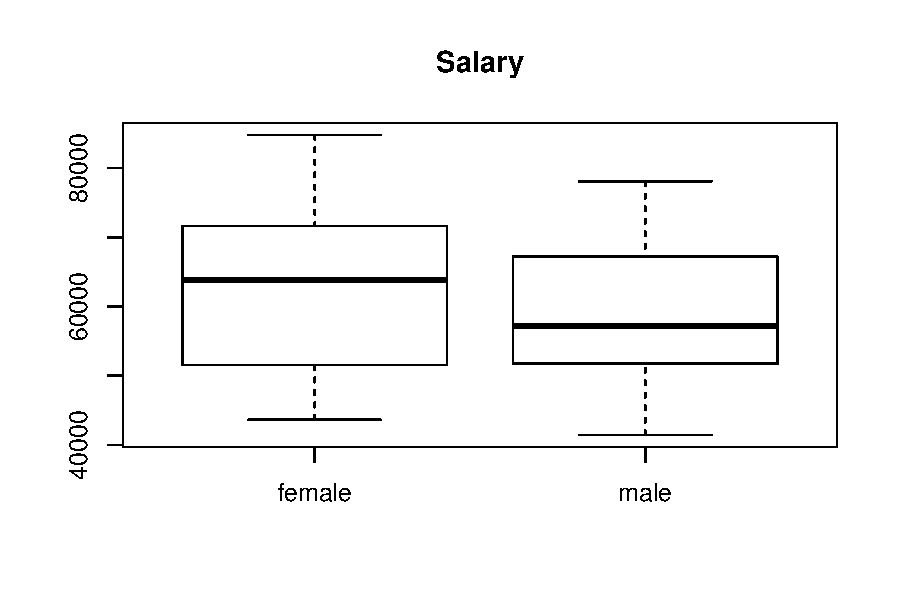
\includegraphics[scale=0.75]{final_May_2017_boxplot_salary}\\
  \vspace{1em}
  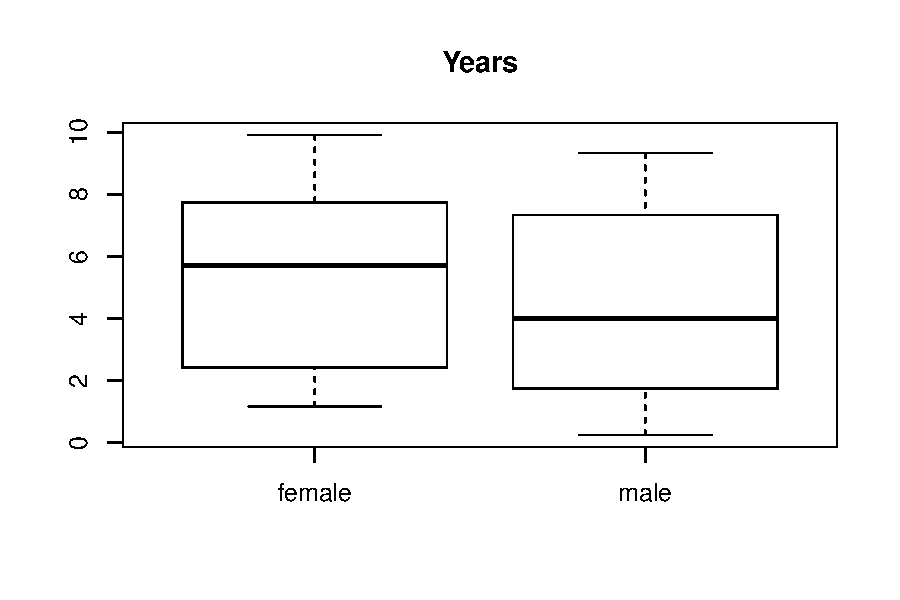
\includegraphics[scale=0.75]{final_May_2017_boxplot_years}\\
\end{figure}

\end{questions}
\end{document}
